\begin{figure}[t]
   \centering
   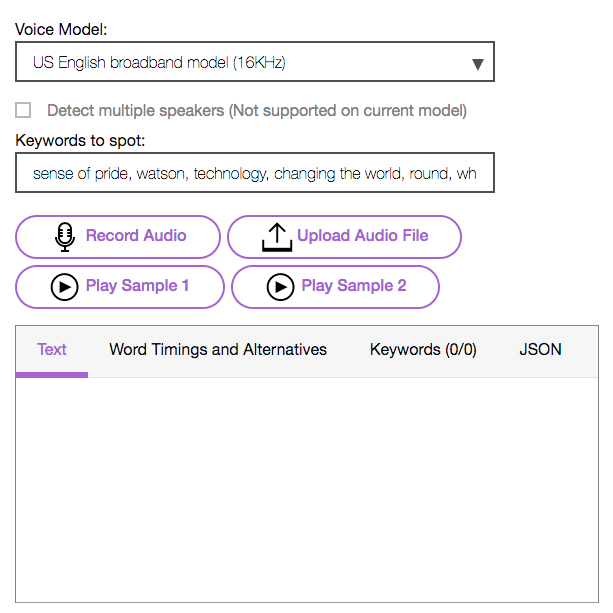
\includegraphics[width=\columnwidth]{figures/ibmwatson.jpg}.
   \caption{IBM Watson's online Speech to Text interface with option to select the Voice Model (accent) and keywords to recognize from the audio. }
   \label{fig:speechrecognizers}
\end{figure}

\section{Initial approach} \mbox{} \
\label{sec:approach}

Before we actually began to implement our system, we tried a few approaches to check the feasibility of our approaches. Using a few of the speech recognition services like Google assistant and Siri, we tried playing the audio files of the CAPTCHAs after downloading them. This approach however failed as the systems were unable to recognize the audio. Next, we tried the possibility of using a mobile application that does specialized speech recognition and it was able to recognize about 2-3 digits from the audio when it was played under a normal room environment. This gave us the motivation that such dedicated speech recognizer would work.\newline

Next, we tried playing the audio from the system while recording it via the microphone at the same time. This had a very poor accuracy, but it led us to the next step, where we rerouted the system audio back to the microphone to mimic the computer talking to itself. This too provided a very poor accuracy. We realized that the real time continuous speech recognition libraries were poor in accuracy in recognizing the audio CAPTCHAs. This led us to explore speech recognition from audio files. \newline

Our next approach was to manually upload these files to speech recognition service that transcribed audio files. We used the IBM Watson's Speech to Text service and were able to transcribe the audio file. The accuracy was not much, but it did provide a few alternative transcriptions, which had the correct values. This indicated that our attack was feasible by using these Speech to Text converters.